% Summary of what we are about to describe
In this chapter, we first describe the {\sc BoSs} memory which contains the dialog history and KB tuples, followed by how the memory is consumed by the encoder and the decoder. We then define the loss function, which, along with dropout, enables disentangled learning of language and knowledge. Finally we go on to explain the RL-decoder and its integration in the \sys -RL architecture.

\section{The \sys\ Architecture}
% Quick Intro
The proposed Bag-of-Sequences Memory Network has an encoder-decoder architecture that takes as input (1) dialog history, which includes a sequence of previous user utterances $\{c_1^u, \ldots, c_{n}^u\}$ and system responses $\{c_1^s, \ldots, c_{n-1}^s\}$, and (2) KB tuples $\{kb_1, \ldots, kb_{N}\}$. The network then generates the next system response $c_n^s=\langle y_1 y_2 \ldots y_T \rangle$ word-by-word. The simplified architecture of \sys\ is shown in Figure \ref{fig:simsystem} and a more detailed architecture is shown in \ref{fig:fullsystem}.
%The network maintains the dialog history and KB tuples in the {\em Bag-Of-Sequences memory}.
% Notations Used

\begin{figure}[t]
\centering
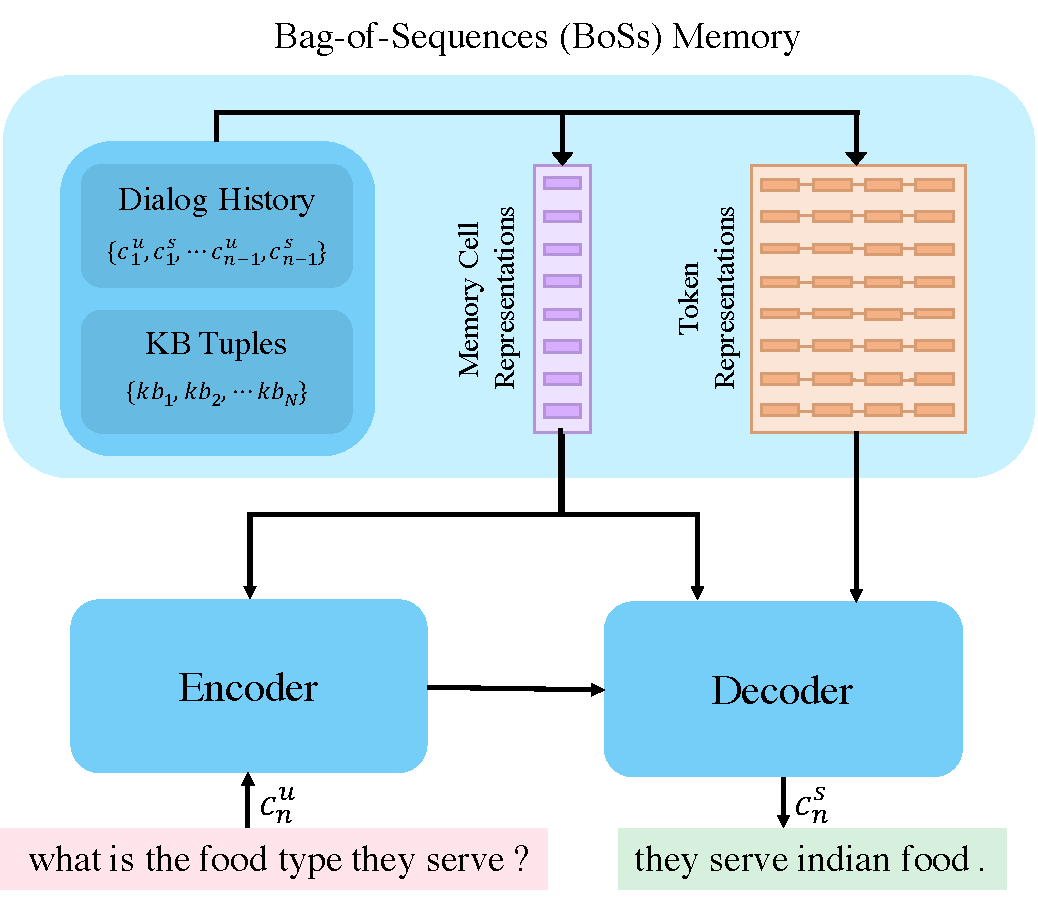
\includegraphics[scale=0.5]{assets/paper_arch.pdf}
\caption{The dialog history and KB tuples stored in the memory have memory cell representations and token representations. The encoder understands the last user utterance using only the memory cell representations. The decoder generates the next response using both representations.}
\label{fig:simsystem}
\end{figure}

\begin{figure}
\centering
\begin{subfigure}{0.8\textwidth}
 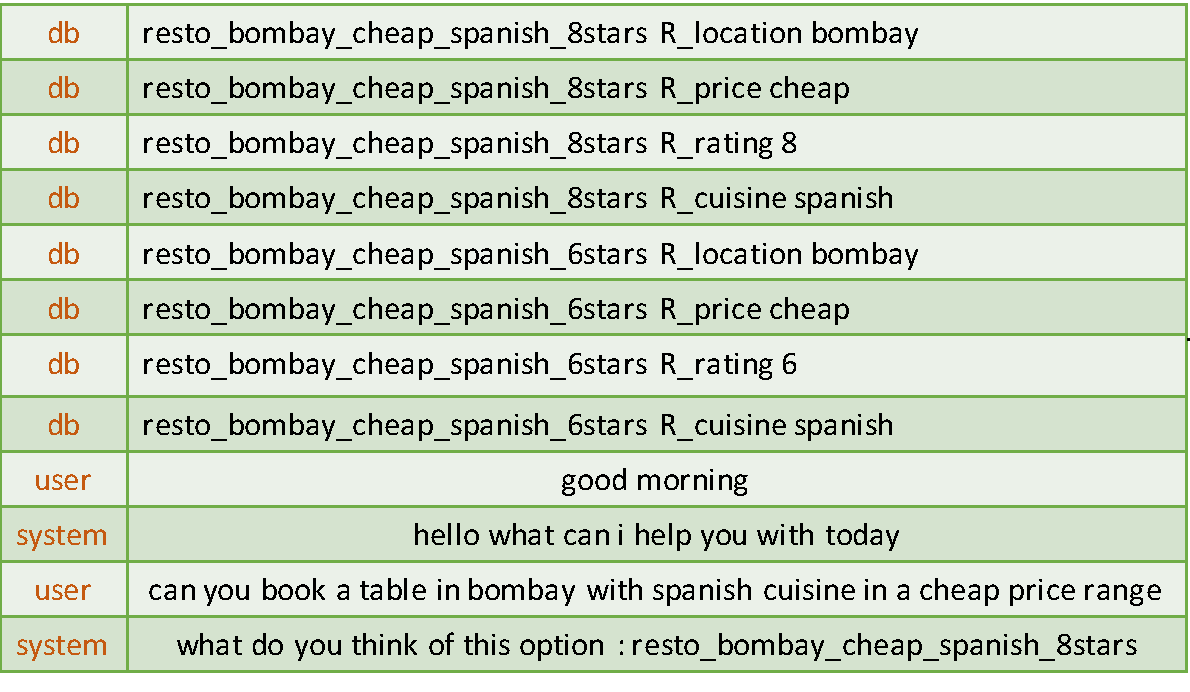
\includegraphics[width=\linewidth]{assets/figures/memory_flat.pdf}
 \caption{Simple Memory Representation (Sentence Level)}\label{fig:flatMemory}
\end{subfigure}

\vspace*{0.5in}

\begin{subfigure}{0.8\textwidth}
 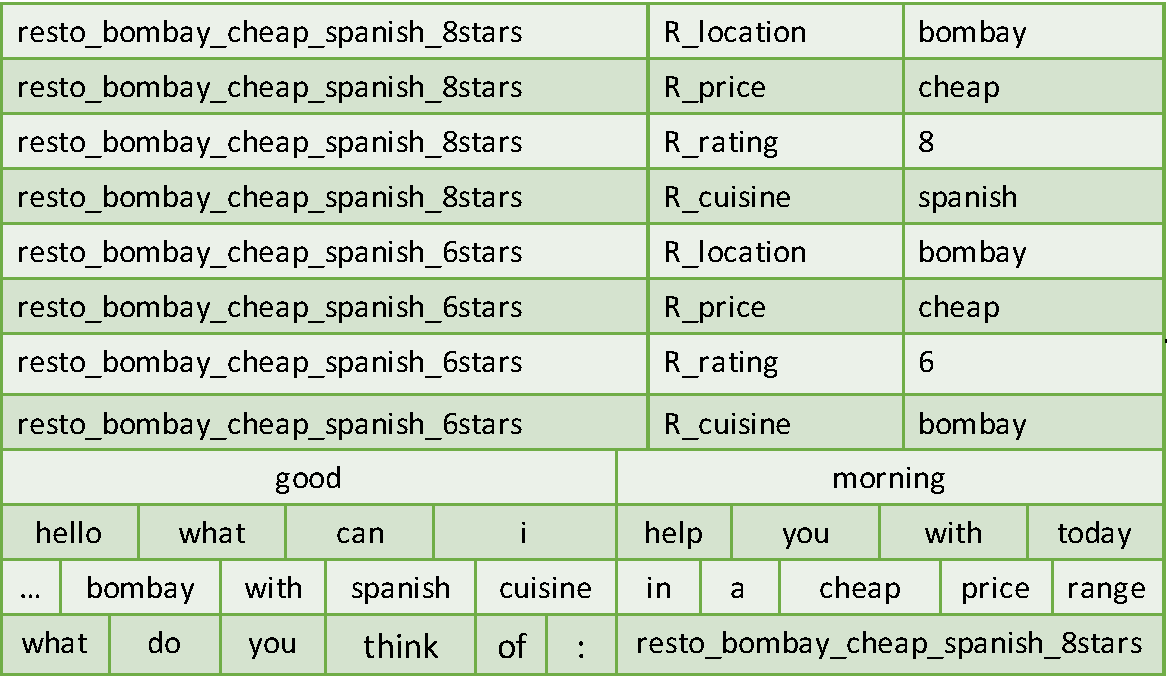
\includegraphics[width=\linewidth]{assets/figures/memory_hier.pdf}
 \caption{{\sc BoSs} Memory Representation (Sentence + Word Level)}\label{fig:hierMemory}
\end{subfigure}
\caption{Types of Memory Architectures}
\end{figure}

\begin{figure}[t]
\centering
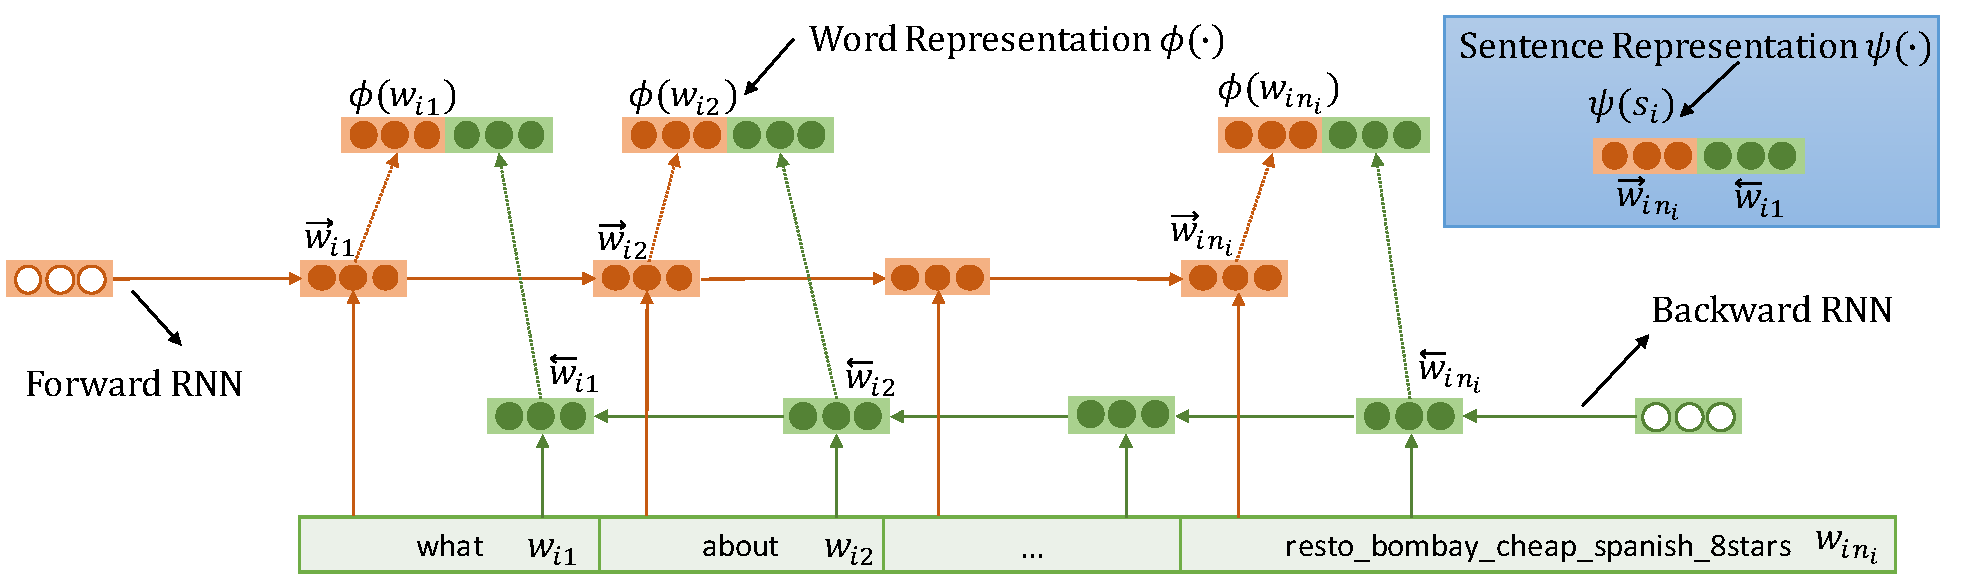
\includegraphics[scale=0.5]{assets/figures/embedding.pdf}
\caption{Each sentence is passed through a bi-directional GRU. We obtain word level embeddings $\phi(w_i)$ and sentence level embeddings $\psi(s_i)$ by concatinating the result of the front and back passes.}
\label{fig:embed}
\end{figure}

\subsection{Bag-of-Sequences Memory} 
\label{sec:hmemory}
The context memory $M$ contains the dialog history $\{c_1^u, c_1^s, \ldots, c_{n-1}^u, c_{n-1}^s\}$ and the KB tuples $\{kb_1, \ldots, kb_{N}\}$. Each utterance in the dialog history and each KB tuple is placed in a memory cell as seen in Figure \ref{fig:hierMemory}. As utterances and tuples are inherently a sequence, we represent each memory cell $m_i$ as an ordered sequence of tokens $\langle w^1_i w^2_i \ldots w^{|m_i|}_i\rangle$. For an utterance, the word tokens are followed by a temporal indicator and a speaker indicator \{\$u (for user), \$s (for system)\}. For example, \{\texttt{good, morning, \#1, \$s}\}\ indicates this was the first utterance by the system. For a KB tuple, the tokens are sequenced as \{\textit{subject, predicate, object}\} followed by temporal indicator and a kb indicator (\texttt{\$db}).

Token representation is generated using a bidirectional GRU. Let the outputs of the forward and backward GRUs for the token $w^j_i$ be denoted as $\overrightarrow{h^j_{i}}$ and $\overleftarrow{h^j_{i}}$ respectively. Then the token representation $\phi(w^j_i)$ is given by Eq. \ref{eqn:1}. Memory cell representation $\psi(m_i)$ is computed by concatenating the forward GRU output of its last token and the backward GRU output of its first token as in Eq. \ref{eqn:2}. This is further visualised in Figure \ref{fig:embed}
\begin{eqnarray}
\phi(w^j_i)=[\overrightarrow{h^j_{i}};\overleftarrow{h_{i}^j}] \label{eqn:1} \\
\psi(m_i)=[\overrightarrow{h_{i}^{|m_i|}};\overleftarrow{h_{i}^1}] \label{eqn:2}
\end{eqnarray}

\begin{figure}[t]
\centering
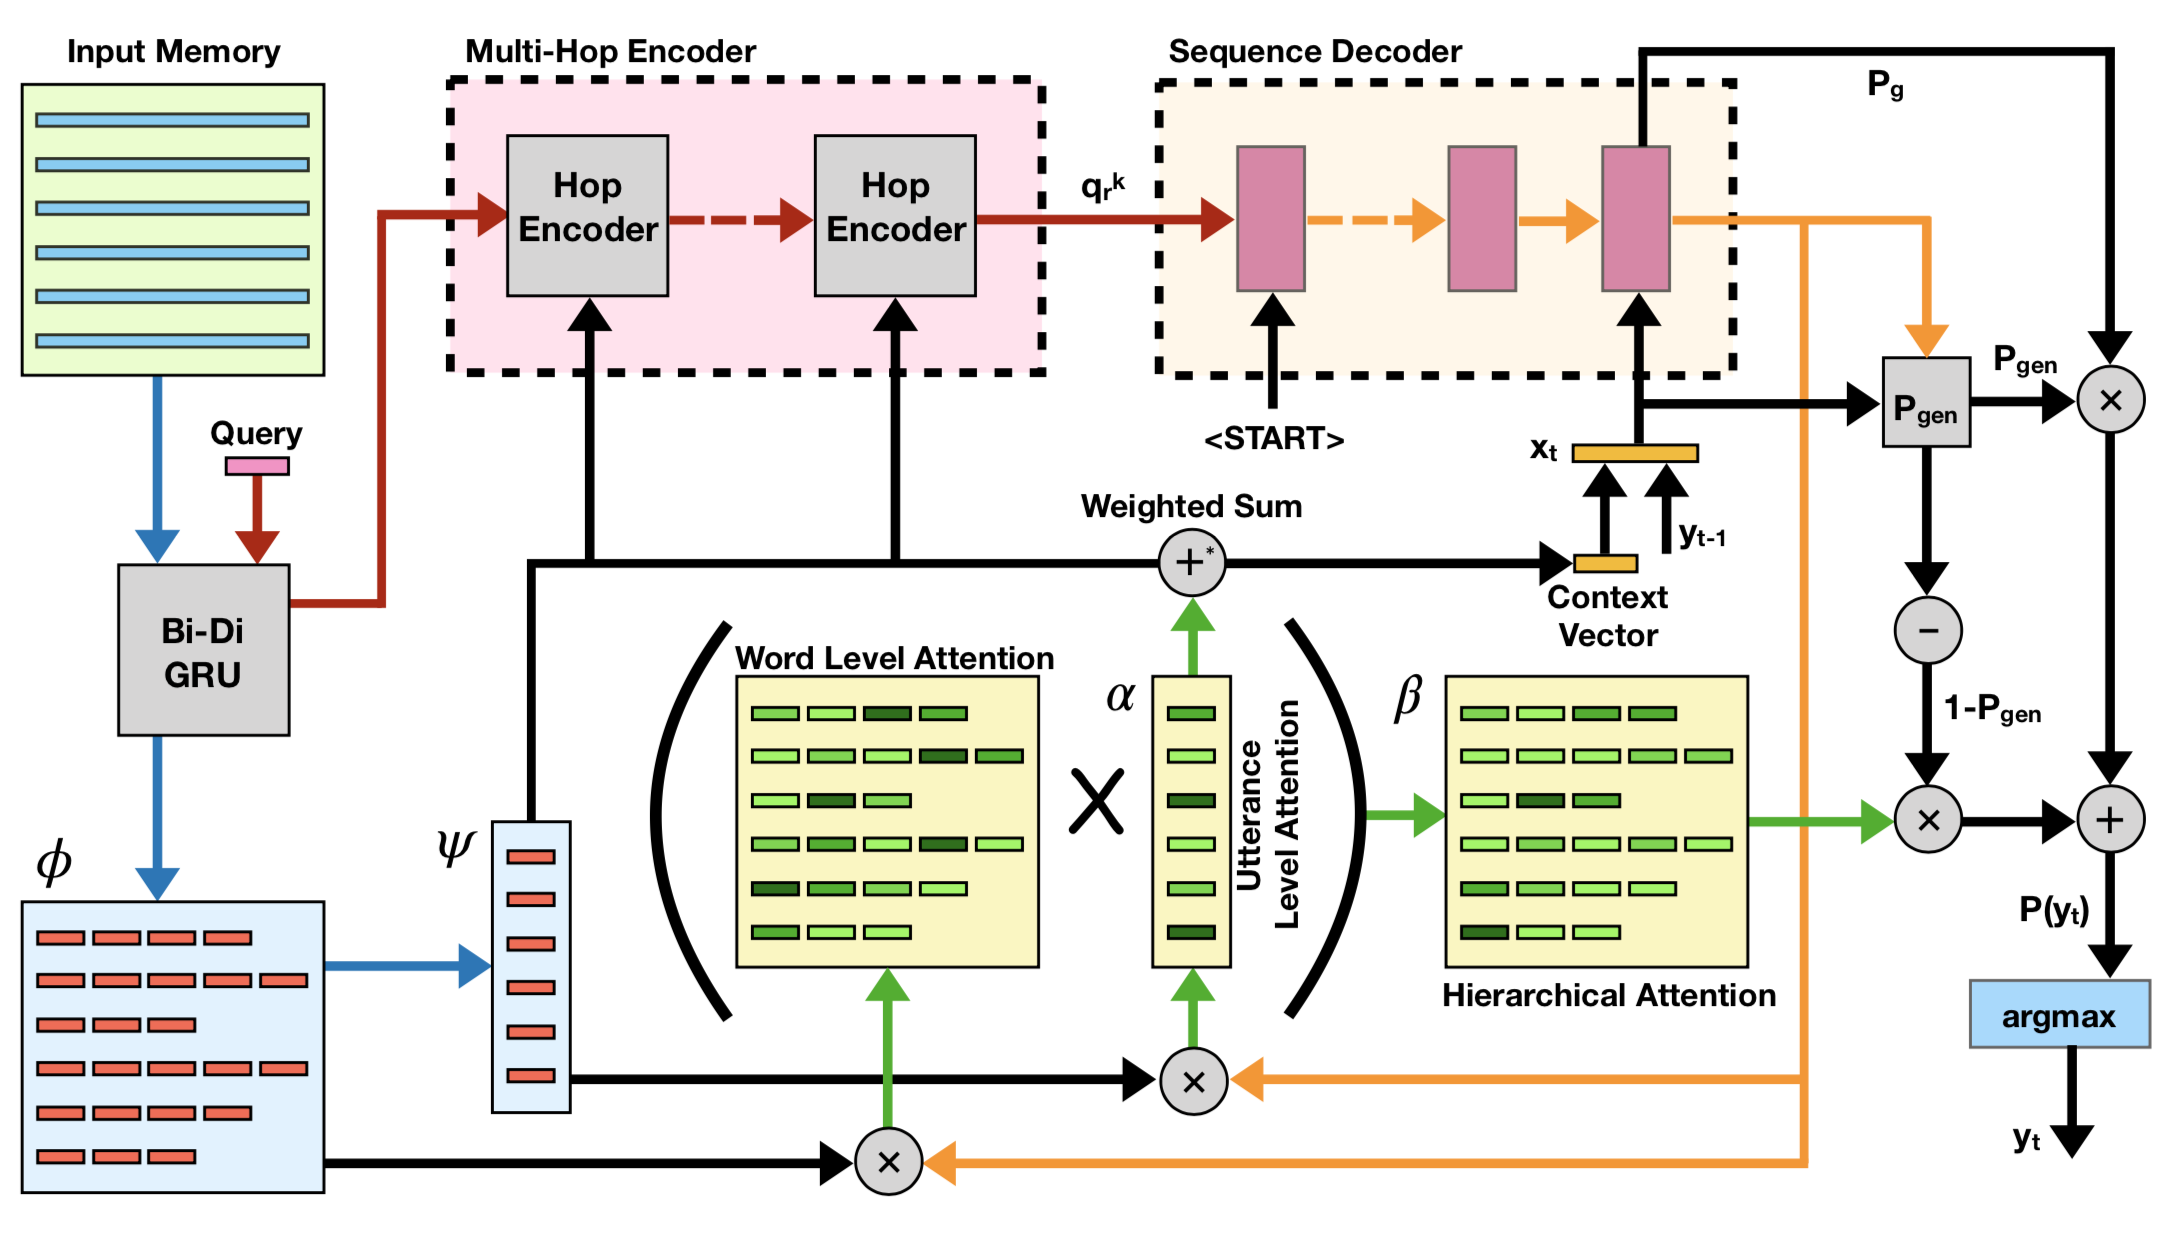
\includegraphics[scale=0.4]{assets/paper_arch.png}
\caption{The detailed encoder-decoder architecture of \sys\ depicting attention over its hierarchical memory and implementation of its copy mechanism.}
\label{fig:fullsystem}
\end{figure}

%\textcolor{blue}{The encoder uses only the memory cell representations to summarize the dialog history and the KB, while the decoder peaks at both the memory cell representation and the token representations during each decode step.}\todo{[N: This is unclear]}

\subsection{The \sys\ Encoder}
\label{ssec:encoder}

The encoder used in \sys\ is similar to the multi-hop attention encoder with layer-wise weights proposed by \cite{sukhbaatar2015end}. The encoder in \cite{sukhbaatar2015end} uses two different embedding matrices, whereas we use just one to reduce the number of parameters. The encoder considers the last user utterance as the query $q=\psi(c_n^u)$ and computes the reduced representation $q_r$ using the memory $M$ as follows:
\begin{eqnarray}
p_i &=& \text{softmax}(q^T \psi(m_i)) \\
o &=& W_r \sum\nolimits_i p_i \psi(m_i) \\
q_r &=& o + W_o q
\end{eqnarray}

where $W_r, W_o \in \mathbb{R}^{d \times d}$ are learnable parameters. The hop step can be re-iterated, by assigning the output of the previous hop as the new input query, i.e., setting $q=q_r$. The output of the encoder after $K$ hops, $q_r^k$, is assigned as the initial state of the decoder.

\subsection{The \sys\ Decoder}
\label{ssec:decoder}

\sys\ models a copy-augmented sequence decoder, which generates the response one word at a time. At any decode time step $t$, the decoder can either \emph{generate} a word from the decode vocabulary or \emph{copy} a word from the memory. Consequently, the decoder computes: (1) generate distribution $P_g(y_t)$ over the decode vocabulary, and (2) copy distribution $P_c(y_t)$ over words in the memory. 

The generate distribution is computed using a standard sequence decoder \cite{sutskever2014sequence} by attending \cite{luong2015effective} over the memory cell representations $\psi$. The copy distribution is generated by using a \textit{two-level attention} over the {\sc BoSs} memory. Given the decoder state $s_t$, it first computes attention $\alpha_t$ over the memory cells. Then it computes attention over the tokens in each memory cell $m_i$. Finally it multiplies both these attentions to compute $P_c(y_t)$ as follows: 
\begin{gather}
\alpha_i^t = \text{softmax}(s_t \psi(m_i)) \\
e_{ij}^t = s_t \phi(w_i^j) \\
\beta^{t}_{ij} = \alpha^t_i * \frac{\exp({e_{ij}^t})}{\sum\nolimits_{k}\exp({e_{ik}^t})} \\
%\beta^{t}_{ij} = \alpha^t_i * \sigma(e_{ij}^{t}) \\
P_c(y_t=w)=\sum_{ij:w_i^j=w} \beta_{ij}^{t}
\end{gather}

%\textcolor{blue}{where $W^w_l, W^u_l \in \mathbb{R}^{d \times d}$ are learnable parameters.}
%\todo{[N: I think we dont use the weight matricies for attention due to extra parameters and low performance.]}

The copy and generate distributions are combined using a soft gate $g_s^t \in [0,1]$ as in \cite{see2017get}. $g_s^t$ is a function of the decoder state at time $t$ and the previous decoded word.

\subsection{Loss}
The decoder is trained using cross-entropy loss. The loss per response is defined as:
\begin{equation}
\mathcal{L}_{ce} = - \sum_{t=1}^{T} \textup{log} \Big( g_s^{t}P_g(y_t) + (1-g_s^{t})P_c(y_t) \Big) 
%\\ + \gamma \sum_{t=1}^{T}H(p^{(t)}_{gen}, p^{(t)}_{ref-gen}) 
\end{equation}
where $T$ is the number of words in the sequence to be generated and $y_t$ is the word to be generated at time step $t$. The decision to generate or copy is learnt implicitly by the network. However, to attain perfect disentanglement, the KB words should be copied, while the language should be generated. In other words, any word in the response that is present in the {\sc BoSs} KB memory should have a low $g_s$. To obtain this behavior, we define a disentangle label $D_{l}$ for each word in the response. This label is set to $1$ if the word is present in the {\sc BoSs} KB memory and $0$ otherwise.
We define a disentangle loss as follows:
\begin{equation}
\mathcal{L}_{d} = - \sum_{t=1}^{T} g_s^{t}\textup{log}D^{t}_{l} + (1-g_s^{t})\textup{log}(1-D^{t}_{l})
\end{equation}

We randomly drop some words with disentangle label set to $1$. This \textit{Disentangle Label Dropout (DLD)} works in tandem with the disentangle loss and {\sc BoSs} memory -- it encourages the model to copy KB words whenever possible, based on their surrounding words. The overall loss is given as:
\begin{equation}
\mathcal{L} = \mathcal{L}_{ce} + \gamma \mathcal{L}_{d}
\label{eqn:loss}
\end{equation}

The relative weight of $\mathcal{L}_{d}$ in the overall loss is controlled using a hyper-parameter ($\gamma$). The dropout rate is also a hyper-parameter.

\section{The \sys -RL Architecture}
The reinforment learning based API generation system builds upon the original \sys\ architecture with added modules (1) API Explorer and (2) RL-decoder. We explain these in the following sections.

\subsection{API Explorer}
This module has the objective of aiding the exploration of valid APIs with a strong reward. Our actual reward for a generated API is implicit, because it depends on the responses of the response model based on the results queried by the API. Hence, we go on to define a psuedo reward for each API as the following:

\noindent\textbf{Psudo Reward}
\label{ssec:PsReward}
The responses by the system depend on the results fetched by the API from the KB. The system will only be able to copy KB information into its response limited to these results. Hence we can measure the performance of a certain API by checking the overlap of the information required by the responses and that present in its results. We use the popular F1 metric which is a combination of precision and recall. For us recall is important because it measures the extent of overlap and the precision will make sure that the results retrieved say as concise as possible. We don't want to have a very generic API which results in a very large result set!. Our metric which we term as the {\em Psuedo Reward} is calculated as follows.
\begin{gather}
Reward = \frac{2 \cdot R \cdot P}{(R + P)}
\end{gather}
where $P$ = No. of KB items in both results and responses / No. of KB items in results \\ and $R$ = No. of KB items in both results and responses / No. of KB items in responses

Our API Explorer then tries to find (explore) valid APIs/queries with a large psuedo-reward to aid in augmented REINFORCE. Taking insiration from \cite{NIPS2018_8204} we maintain a buffer of the best APIs found during this exploration phase which runs before and during training.

\subsection{RL-decoder}
\label{ssec:rldecode}
The RL-decoder is added as a second decoder to the \sys\ architecture. It is activated when the system receives a {\em Make API} command. It uses a different embedding matrix from the original encoder to encode the context which serves as the initial state to the encoder. The decoder uses a sequence independence approach to generate the output akin to a slot-filling technique with a fixed template. This style of decoding mitigates the length bias problem associated with RL generation. The initial state is passed on at each timestep of the decode process and only the current timestep is given as input. This makes each decode step independent of the previously decoded sequence and it is completely focused on finding the correct information in the context to fill in its current slot/timestep.
\begin{gather}
s_{t} = (s,t)
\end{gather}